\documentclass{mini}

% PACKAGES
%------------------------------------------------------------------------------%
\usepackage[utf8]{inputenc}
\usepackage{tikz}
\usepackage{pgfplots}
\usepackage{wrapfig}

\usepackage{csquotes}
\usepackage{amsmath}
\usepackage{epigraph}
\usepackage[linesnumbered,ruled]{algorithm2e}
\usepackage{adjustbox}

\DeclareMathOperator*{\argmin}{arg\,min} %argmin
\DeclareMathOperator*{\argmax}{arg\,max} %argmax

\usepackage{floatrow}
% Table float box with bottom caption, box width adjusted to content
\newfloatcommand{capbtabbox}{table}[][\FBwidth]
\usepackage{caption}
\usepackage{subcaption}
\captionsetup{compatibility=false}

%%%

\usepackage{array}
% For tabulars
\newcolumntype{P}[1]{>{\centering\arraybackslash}p{#1}}


\usepackage{pdfpages}
\usepackage{graphicx}
\usepackage{longtable}
%\usepackage[export]{adjustbox}
%\usepackage{tabu}
\usepackage{xcolor,colortbl}
\usepackage{caption}
\usepackage{subcaption}
\usepackage{float}
\usepackage{wrapfig}
\usepackage{amsfonts}


% TITLE
%------------------------------------------------------------------------------%
\title{Bachelor Exam}
\titleaux{}
\author{Jakub Ciecierski}

\supervisor{Jezus}
\type{bachelor}
\discipline{Computer Science}
\monthyear{february 2016}
\date{\today}
\album{243260}

%------------------------------------------------------------------------------%

\begin{document}
\maketitle
\tableofcontents

%---------------------------------------------------------------
\chapter{Algorithm Design and Complexity}

%---------------------------------------------------------------
\chapter{Graph Theory}

%---------------------------------------------------------------
\chapter{Automata Theory and Languages}

%---------------------------------------------------------------
\chapter{Numerical Methods}

%---------------------------------------------------------------
\chapter{Programming}

%---------------------------------------------------------------
\chapter{Computer Graphics}

Sources: \cite{phong}, \cite{lighting}

%---------------------------------------------------------------
%---------------------------------------------------------------
\section{Color Models}



%---------------------------------------------------------------
%---------------------------------------------------------------
\section{Illumination Models}


Illumination Models can be split into two groups:
\begin{itemize}
    \item {\bf Local.}
    \begin{itemize}
        \item Objects are considered independently. Direct Reflections.
        \item Tries to mimic reality with the small computational complexity
        \item Example: {\bf Phong Illumination}
    \end{itemize}
    
    \item {\bf Global.}
    \begin{itemize}
        \item Light reflected from other objects
        \item Closer to reality, requires big computational complexity 
        \item Example: {\bf Ray Tracing, Radiosity.}
    \end{itemize}
\end{itemize}

\subsection{Phong Illumination}

\begin{figure}[H]
    \centering
    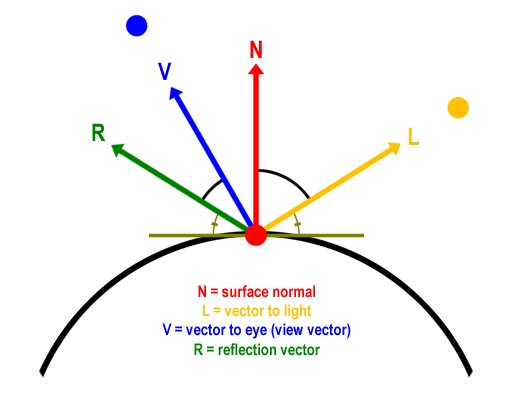
\includegraphics[width=0.8\textwidth]{./images/phong.jpg}
    \caption{}
    \label{fig:phong}
\end{figure}

Phong illumination specifies the four vectors described in figure~\ref{fig:phong} and several colors:

\begin{itemize}
    \item $A_L$, $A_M$ - Ambient color of the light source and surface material
    \item $D_L$, $D_M$ - Diffuse color of the light source and surface material
    \item $S_L$, $S_M$ - Specular color of the light source and surface material
\end{itemize}

Because light is additive, the final intensity of the light reflected by a given surface is simply the sum of the ambient, diffuse and specular components:
\begin{center}
    $I = A + D + S$
\end{center}



%---------------------------------------------------------------
%---------------------------------------------------------------
%---------------------------------------------------------------
\subsection{Ambient Light}
Ambient light is a constant amount of light that gets added to the scene no matter what. It's goal is to fake the contribution of indirect reflections, which can normally only be accounted for using global illumination solutions. The ambient term is used simply to keep shadows from turning pitch black, which would be very unrealistic.

{\bf Ambient light is a "hack" to simulate global illumination.}



\begin{figure}[H]
    \centering
    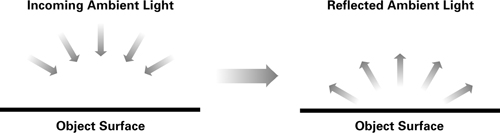
\includegraphics[width=1.0\textwidth]{./images/ambient_light.jpg}
    \caption{}
    \label{fig:ambient}
\end{figure}

{\bf The ambient term is simply a combination of the ambient components of the light source and the surface material.} By multiplying the light color and the material color, we account for the fact that any material only reflects certain frequencies of light. A green surface, for example, does not reflect red light. As we will see below, the diffuse and specular terms also combine the light and material colors in the same way.

\begin{center}
    $A = A_L \cdot A_M$
\end{center}

%---------------------------------------------------------------
%---------------------------------------------------------------
%---------------------------------------------------------------
\subsection{Diffuse Light}
The diffuse term accounts for directed light reflected off a surface equally in all directions. In general, diffuse surfaces are rough on a microscopic scale, with small nooks and crannies that reflect light in many directions. When incoming rays of light hit these nooks and crannies, the light bounces off in all directions

\begin{figure}[H]
    \centering
    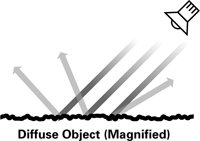
\includegraphics[width=0.5\textwidth]{./images/diffuse_magnified.jpg}
    \caption{Intuition behind the diffuse light. The magnified object has alot of nooks and crannies, thus the lights bounces off in all directions}
    \label{fig:diffuse_magnified}
\end{figure}

The amount of light reflected is proportional to the angle of incidence of the light striking the surface. Surfaces with a dull finish, such as a dusty chalkboard, are said to be diffuse. The diffuse contribution at any particular point on a surface is the same, regardless of where the viewpoint is.

{\bf Diffuse light hits a surface and gets scattered equally into all directions}

\begin{figure}[H]
    \centering
    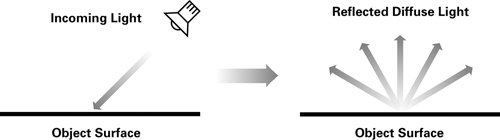
\includegraphics[width=1.0\textwidth]{./images/diffuse.jpg}
    \caption{}
    \label{fig:diffuse}
\end{figure}

{\bf Diffuse lighting is based on the angle between the light vector and the surface normal.} The surface normal is a given, and requires no further explanation. The light vector L is the normalized vector from the point being shaded to the light source. Given these two vectors, the diffuse term is:

\begin{center}
    $ D = D_L \cdot D_M \cdot max(L \bullet N, 0) $
\end{center}

The dot product of L and N returns the cosine of the angle between those two vectors. When the two vectors are equal, the dot product is one. When they are perpendicular, the value is zero. If the two vectors point away from each other, the value becomes negative. When this happens, the value must be clamped to zero to prevent ending up with "negative light".

The clamped dot product is also multiplied (or modulated) with the diffuse colors of the light and the surface material.


%---------------------------------------------------------------
%---------------------------------------------------------------
%---------------------------------------------------------------
\subsection{Specular Light}

{\bf The specular term represents light scattered from a surface predominantly around the mirror direction.} The specular term is most prominent on very smooth and shiny surfaces, such as polished metals.

\begin{figure}[H]
    \centering
    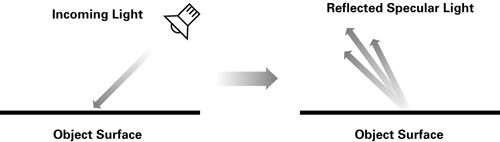
\includegraphics[width=1.0\textwidth]{./images/specular.jpg}
    \caption{}
    \label{fig:specular}
\end{figure}

{\bf Specular term is dependent on the angle between the reflected light vector R and the view vector V.} The view vector is the normalized vector from the point being shaded to the camera position. The reflection vector is calculated as follows:

\begin{center}
    $ R = 2(N \bullet L) N-L$
\end{center}

{\bf The reflection vector represents the direction the incoming light would be reflected in if the surface were a perfect mirror}. The angle between R and N is equal to that between L and N. Having calculated R and V, we can now compute the specular term:

\begin{center}
    $ S = S_L \cdot S_M \cdot max(R \bullet V, 0)^{n} $
\end{center}

The dot product is there because we want to favor reflections in the direction of the camera to those that point away from the camera. The larger the angle between R and V, the lower the specular term will be. Notice how we also raise the dot product to a power of n, where n is called the specular exponent of the surface and represents its shininess. Higher values of n lead to smaller, sharper highlights, whereas lower values result in large and soft highlights

To summarize Specular Light:
\begin{itemize}
    \item reflection off of shiny surfaces - you see a highlight
    \item shiny metal or plastic has high specular component
    \item chalk or carpet has very low specular component
    \item position of the viewer IS important in specular reflection
\end{itemize}


{\bf Remark:} Blinn Specular uses half-angle vector which is a vector halfway between the light vector and the view vector


\subsection{Summary}

\begin{figure}[H]
    \centering
    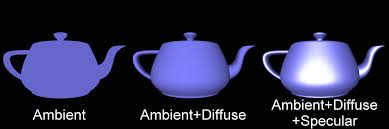
\includegraphics[width=0.8\textwidth]{./images/phong_components.jpg}
    \caption{}
    \label{fig:phong_components}
\end{figure}


%---------------------------------------------------------------
%---------------------------------------------------------------
\section{Shading}

\subsection{Flat Shading}
\begin{itemize}
    \item Each entire polygon is drawn with the same color
    \item Need to know one normal for the entire polygon
    \item Fast
    \item Lighting equation used once per polygon
\end{itemize}

\begin{figure}[H]
    \centering
    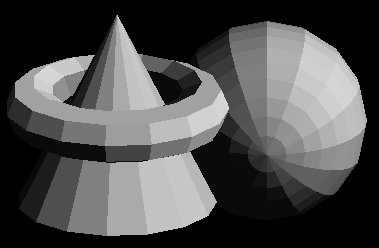
\includegraphics[width=0.5\textwidth]{./images/flat_shade.jpg}
    \caption{}
    \label{fig:flat_shade}
\end{figure}


\subsection{Goraud Shading}
First, intensities on vertices are calculated. Then color at each pixel inside a polygon is a linear interpolation of intensities at vertices
\begin{itemize}
   
    \item Colors are interpolated across the polygon
    \item Need to know a normal for each vertex of the polygon
    \item Slower than flat shading
    \item Lighting equation used at each vertex
\end{itemize}

\begin{figure}[H]
    \centering
    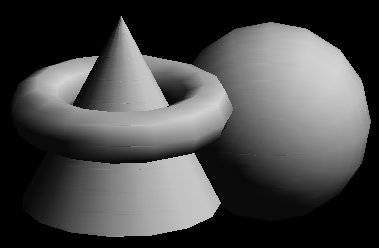
\includegraphics[width=0.5\textwidth]{./images/goraud_shade.jpg}
    \caption{}
    \label{fig:goraud_shade}
\end{figure}

\subsection{Phong Shading}

\begin{itemize}
    \item Normals are interpolated across the polygon
    \item Need to know a normal for each vertex of the polygon
    \item Better at dealing with highlights than Goraud shading
    \item Slower than Goraud shading
    \item Lighting equation used at each pixel
\end{itemize}
Where Goraud shading uses normals at the vertices and then interpolates the resulting colours across the polygon, Phong shading goes further and interpolates tha normals. Linear interpolation of the normal values at each vertex are used to generate normal values for the pixels on the edges. Linear interpolation across each scan line is used to then generate normals at each pixel across the scan line.


%---------------------------------------------------------------
%---------------------------------------------------------------
\section{Raster Algorithms}

A line drawing algorithm is a graphical algorithm for approximating a line segment on discrete graphical media. On discrete media, such as pixel-based displays and printers, line drawing requires such an approximation (in nontrivial cases). Basic algorithms rasterize lines in one color. A better representation with multiple color gradations requires an advanced process, anti-aliasing.

%---------------------------------------------------------------
%---------------------------------------------------------------
%---------------------------------------------------------------
\subsection{Line Drawing}

Naive line drawing uses floating point operations which is slowing down the computations

\subsubsection{Bresenham}
{\bf Midpoint line algorithm}

We choose E or NE by calculating on which side of the line the mid point lies

\begin{figure}[H]
    \centering
    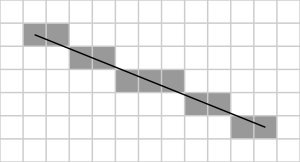
\includegraphics[width=0.5\textwidth]{./images/bresenham.png}
    \caption{}
    \label{fig:bresenham}
\end{figure}


%---------------------------------------------------------------
%---------------------------------------------------------------
%---------------------------------------------------------------
\subsection{Aliasing and Anti-Aliasing}

Bresenham yields a aliased line: appearing stepped or jagged.

\begin{figure}[H]
    \centering
    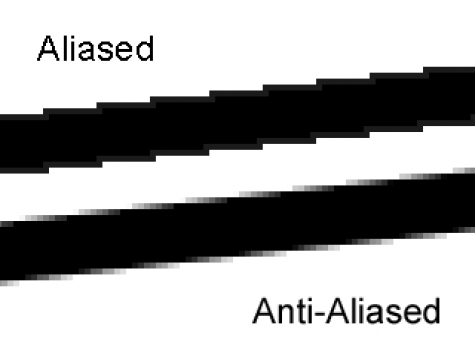
\includegraphics[width=0.5\textwidth]{./images/aliasing.png}
    \caption{}
    \label{fig:aliasing}
\end{figure}


%---------------------------------------------------------------
%---------------------------------------------------------------
\section{Spline Functions}

%---------------------------------------------------------------
%---------------------------------------------------------------
\section{Filling the Area}

%---------------------------------------------------------------
%---------------------------------------------------------------
\section{Visible Surface Determination}

%---------------------------------------------------------------
%---------------------------------------------------------------
\section{Image Filtering}

%---------------------------------------------------------------
\chapter{Software Engineering}


%---------------------------------------------------------------
\begin{thebibliography}{1}
\bibitem{phong} $http://www.gameprogrammer.net/delphi3dArchive/phongfordummies.html$

\bibitem{lighting} $http://http.developer.nvidia.com/CgTutorial/cg_tutorial_chapter05.html$

\end{thebibliography}


\end{document}
